
%% bare_conf.tex
%% V1.3
%% 2007/01/11
%% by Michael Shell
%% See:
%% http://www.michaelshell.org/
%% for current contact information.
%%
%% This is a skeleton file demonstrating the use of IEEEtran.cls
%% (requires IEEEtran.cls version 1.7 or later) with an IEEE conference paper.
%%
%% Support sites:
%% http://www.michaelshell.org/tex/ieeetran/
%% http://www.ctan.org/tex-archive/macros/latex/contrib/IEEEtran/
%% and
%% http://www.ieee.org/

%%*************************************************************************
%% Legal Notice:
%% This code is offered as-is without any warranty either expressed or
%% implied; without even the implied warranty of MERCHANTABILITY or
%% FITNESS FOR A PARTICULAR PURPOSE! 
%% User assumes all risk.
%% In no event shall IEEE or any contributor to this code be liable for
%% any damages or losses, including, but not limited to, incidental,
%% consequential, or any other damages, resulting from the use or misuse
%% of any information contained here.
%%
%% All comments are the opinions of their respective authors and are not
%% necessarily endorsed by the IEEE.
%%
%% This work is distributed under the LaTeX Project Public License (LPPL)
%% ( http://www.latex-project.org/ ) version 1.3, and may be freely used,
%% distributed and modified. A copy of the LPPL, version 1.3, is included
%% in the base LaTeX documentation of all distributions of LaTeX released
%% 2003/12/01 or later.
%% Retain all contribution notices and credits.
%% ** Modified files should be clearly indicated as such, including  **
%% ** renaming them and changing author support contact information. **
%%
%% File list of work: IEEEtran.cls, IEEEtran_HOWTO.pdf, bare_adv.tex,
%%                    bare_conf.tex, bare_jrnl.tex, bare_jrnl_compsoc.tex
%%*************************************************************************
%

\documentclass[conference]{IEEEtran}
%\usepackage{draftcopy}

\usepackage{graphicx}
\usepackage{color}
\usepackage{multirow}


%\graphicspath{{fig/}}
\newcommand \todo[1]{\textcolor{red}{\textsl{TODO: }}{\textcolor{black}{#1}}}
\newcommand \modified[1]{{\textcolor{black}{#1}}}
\newcommand \attention[1]{{\textcolor{black}{#1}}}
%\renewcommand{\thefootnote}{\alph{footnote}}
\hyphenation{op-tical net-works semi-conduc-tor}

\graphicspath{ {../../figures/} }

\begin{document}

\title{Performance results of the first White Rabbit installation for CNGS 
        \footnote{CERN Neutrinos to Gran Sasso}time transfer  }

% author names and affiliations
% use a multiple column layout for up to three different
% affiliations

\author{

%\IEEEauthorblockN{Bunch of Freaks}
%\IEEEauthorblockA{CERN\\
%Geneva\\
%Email: white.rabbit@cern.ch}

\IEEEauthorblockN{Maciej Lipi\'{n}ski, Tomasz W\l{}ostowski, Javier Serrano, Pablo Alvarez}
\IEEEauthorblockA{CERN, Geneva\\
Email: \{maciej.lipinski, tomasz.wlostowski, javier.serrano, pablo.alvarez.sanchez\}@cern.ch}

}

% conference papers do not typically use \thanks and this command
% is locked out in conference mode. If really needed, such as for
% the acknowledgment of grants, issue a \IEEEoverridecommandlockouts
% after \documentclass

% for over three affiliations, or if they all won't fit within the width
% of the page, use this alternative format:
% 
%\author{\IEEEauthorblockN{Michael Shell\IEEEauthorrefmark{1},
%Homer Simpson\IEEEauthorrefmark{2},
%James Kirk\IEEEauthorrefmark{3}, 
%Montgomery Scott\IEEEauthorrefmark{3} and
%Eldon Tyrell\IEEEauthorrefmark{4}}
%\IEEEauthorblockA{\IEEEauthorrefmark{1}School of Electrical and Computer
%Engineering\\
%Georgia Institute of Technology,
%Atlanta, Georgia 30332--0250\\ Email: see
%http://www.michaelshell.org/contact.html}
%\IEEEauthorblockA{\IEEEauthorrefmark{2}Twentieth Century Fox, Springfield,
%USA\\
%Email: homer@thesimpsons.com}
%\IEEEauthorblockA{\IEEEauthorrefmark{3}Starfleet Academy, San Francisco,
%California 96678-2391\\
%Telephone: (800) 555--1212, Fax: (888) 555--1212}
%\IEEEauthorblockA{\IEEEauthorrefmark{4}Tyrell Inc., 123 Replicant Street, Los
%Angeles, California 90210--4321}}


\maketitle

\begin{abstract}

White Rabbit (WR) is a time-deterministic, low-latency Ethernet-based network which enables 
transparent, sub-ns accuracy timing distribution. It is being developed to replace 
the General Machine Timing (GMT) 
%\cite{biblio:GMT} 
system currently used at CERN and will become 
the foundation for the control system of the Facility for Antiproton and Ion Research (FAIR) 
at GSI. High reliability is an important issue in WR's design, 
since unavailability of the accelerator's 
control system will directly translate into expensive downtime of the machine. 
A typical WR network is required to lose not more than a single message per year. 
Due to WR's complexity, the translation of this real-world-requirement into 
a reliability-requirement constitutes an interesting issue on its own -- a WR network 
is considered functional only if it provides all its services to all its clients at any time. 
This paper defines reliability in WR and describes how it was addressed by dividing it into 
sub-domains: deterministic packet delivery, data 
%redundancy, 
resilience, 
topology redundancy and clock 
resilience. The studies show that the Mean Time Between Failure (MTBF) of the WR Network 
is the main factor affecting its reliability. Therefore, probability calculations for 
different topologies were performed using the "Fault Tree analysis" and analytic estimations. 
Results of the study show that the requirements of WR are demanding. Design changes might be needed 
and further in-depth studies required, e.g. Monte Carlo simulations. Therefore, a direction 
for further investigations is proposed.
\end{abstract}


\section{Introduction}

White Rabbit (WR, \cite{biblio:whiteRabbit}) is a project which aims at creating an
Ethernet-based network with low-latency, deterministic packet delivery
and network-wide, transparent, high-accuracy timing distribution. The
White Rabbit Network (WRN) is based on existing standards, namely
Ethernet (IEEE 802.3 \cite{biblio:IEEE8023}), Synchronous Ethernet
(SyncE \cite{biblio:SynchE}) and PTP \cite{biblio:IEEE1588}. 
It is fully compatible with these standards.

A WRN consists of White Rabbit Nodes (nodes) and White Rabbit Switches
(switches) interconnected by fiber or copper links. 
\modified{The focus of this article is on 1000Base-LX \cite{biblio:IEEE1588} 
single-mode fiber connections only. WR }%It also
supports integration of nodes and/or switches that are not White Rabbit. 
A simple WRN is presented in \figurename~\ref{fig:WRnetwork}.

A node is considered the source and destination of information sent
over the WRN. The information distributed over a WRN includes:
\begin{itemize}
   \item  Timing - frequency and International Atomic Time (TAI).
   \item  Data  - Ethernet traffic between nodes.
\end{itemize} 

In order to understand the goals of the WR project -- namely
determinism, high reliability and accurate synchronization -- these
terms are explained below.

\textbf{Determinism} is guaranteed by having a worst-case upper bound
in frame delivery latency.  

\textbf{Accuracy} is a measure of the deviation between the clock of
the \textit{grandmaster} node\modified{/switch} of a WRN and that of any other node.
Assuming only fiber interconnections, a WRN is meant to achieve
sub-nanosecond accuracy. 

\textbf{Reliability} of a WRN refers to robust delivery of data and
timing to all the nodes.
% data being delivered in a deterministic manner. 
%A WRN is considered reliable only if all the nodes, receive
%data and timing. 
The timing must allow all the nodes to be
synchronized with the required accuracy and the data must always be
delivered on time.
\begin{figure}[!t]
\centering
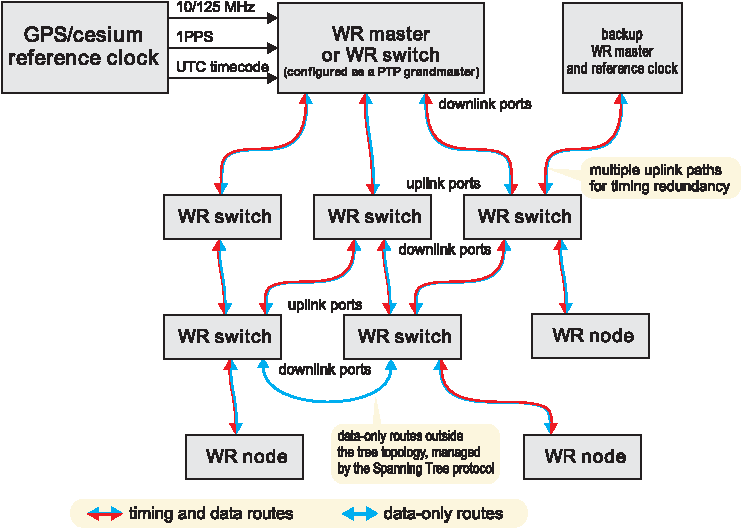
\includegraphics[height=2.10in]{../../figures/network/hierarchy.eps}
\caption{A White Rabbit Network \cite{biblio:TomekMSc}.}
\label{fig:WRnetwork}
\end{figure}

All these features are required to create a timing and control system which may
replace the General Machine Timing (GMT) \cite{biblio:GMT} at CERN and
fulfill a similar role at the Facility for Antiproton and Ion
Research (FAIR) in GSI \cite{biblio:FAIRtimingSystem}. Such system requires 
synchronization of up to 2000 nodes with sub-nanosecond accuracy, 
an upper bound in frame delivery and a very low data loss rate.
However, many other applications of White Rabbit are possible. This includes industry,
telecommunications and other large distributed systems (e.g. distributed
oscilloscopes \cite{biblio:distOscilloscope}).

This article focuses solely on the PTP-based timing distribution in a WRN. PTP is a packet-based
protocol designed to synchronize devices in distributed systems. The accuracy of the PTP
synchronization is implementation-dependent. The standard is foreseen for 
% this is how I understand the fact that corretionField can carry fractional
% nanoseconds and the syncEventEgressTimestamp includes this figures (see e.g.: 
% clause 9.5.9.3, page 103 of PTP
sub-nanosecond accuracies. However, such performance is not achieved in typical PTP
implementations for two reasons:
\begin{itemize}
  \item Limited precision and resolution of PTP timestamps.
  \item Unknown physical link asymmetry. 
\end{itemize}
Additionally, the quality of PTP-syntonization depends on the exchange rate 
of PTP messages. The higher the quality of the clock we want to recover, 
the higher the bandwidth needed for PTP-related traffic.

The precision of timestamps is greatly increased in the existing PTP implementations
by hardware-based timestamping. However, such implementations
are limited by the resolution which is specified by the hardware-driving frequency
(e.g. 8ns for 125MHz).

The asymmetry is not detectable by PTP; if known, PTP corrects for it to increase
synchronization accuracy. Some of the sources of the physical layer asymmetry can be
eliminated by proper network configuration, e.g. excluding routers or non-PTP bridges from the
network. Others, in particular the inaccuracy caused by physical medium asymmetry (i.e.
difference in propagation velocity in two-way communication over fiber) or PCB layout (i.e.
connection length between PHY and timestamping hardware) need to be obtained through proper a
priori-measurement. 

White Rabbit addresses these limitations to achieve sub-nanosecond accuracy
of synchronization. It uses SyncE to distribute the common notion of frequency in the entire
network over the physical medium. It casts the problem of timestamping into a phase detection
measurement. The results of these precise measurements are used both during normal PTP operation
and for quantifying physical medium asymmetry during the calibration phase.
% Consequently, high precision
% timestamps are obtained. Moreover, the parameters necessary to calculate the physical medium
% asymmetry can be determined. 
%This knowledge is used in the PTP computations of the clock offset and link delay. 
The improved performance of the synchronization is accomplished without increasing PTP-related
traffic (it can be actually decreased) since PTP is only governing the synchronization, while the
syntonization is done by SyncE.

A great effort has been made to align WR-specific solutions with the PTP standard and stay fully
compatible with PTP gear. Consequently, WR can be seen as an extension to PTP. This extension,
called WRPTP, defines its own PTP profile and describes all the WR-specific mechanisms which need
to be implemented by a node/switch to enable sub-nanosecond synchronization with another 
nodes/switches. 
\modified{The compatibility with PTP makes WR more likely to be used in existing PTP-based 
systems by gradual and/or partial upgrade to WRPTP. It also enables the creation of hybrid, 
thus cost-effective, systems.}
WRPTP is presented in section~\ref{sec:wrptp} \textit{White Rabbit PTP}.
Section~\ref{sec:hwSupport} presents an example implementation of 
hardware which supports WRPTP. Finally, the measurements of WRPTP performance and conclusions are
presented in the last two sections of this article.

In PTP nomenclature, the main component of a WRN, the switch, is a boundary clock (BC) -- a clock 
that has multiple PTP ports. Similarly, the node is an ordinary clock (OC) --
a clock that has a single PTP port. Consequently, the WRN
can be seen as a set of independently synchronized Master-to-Slave
(M-to-S) links with ports of OC or BC on both sides
(\figurename~\ref{fig:WRnetwork}, red-blue arrows). The ability to
synchronize a single link scales into the ability to synchronize the
entire network. Therefore, in this article, only a single M-to-S link is
considered, where appropriate.




\section{WR deployment, monitoring and test setups}
\label{sec:deplAndMeas}
\subsection{\modified{White Rabbit} in CNGS} 

White Rabbit is used to transfer the UTC timebase from the GPS receiver to the 
measurement point automatically compensating any cable delays and their variation with temperature. 
A~WR setup, both at CERN and LNGS (\figurename~\ref{fig:wrLNGStiming}), consists of WR Switches 
(switches~\cite{biblio:WRswitch}) 
and WR Nodes (nodes) connected with single mode fiber (G.652.B type \cite{biblio:Draka}). % TODO: check the type
The node is a Simple PCIe\footnote{Peripheral Component Interconnect Express} 
FMC\footnote{Field Programmable Gate Array (FPGA) Mezzanine Card} carrier (SPEC) \cite{biblio:spec}
equipped with a Fine Delay FMC module \cite{biblio:fineDelay} which is used as 
a Time-to-Digital Converter (TDC). The TDC time-tags input signals with 28~ps 
resolution, 55~ps precision (std. dev) and 300~ps accuracy \cite{biblio:fineDelay}
with reference to the WR-provided UTC timebase.

A~switch connected to an external time reference (i.e. the switch in the WR Room in 
\figurename~\ref{fig:wrLNGStiming} connected to PPS and 10~MHz inputs) acts as a 
PTP grandmaster. A~switch connected to the grandmaster (directly or through other switches) 
acts as a PTP boundary clock (transparent \modified{clocks are not supported} by WRPTP)
and provides a PPS output synchronized to that of the grandmaster (i.e. the switch in LNGS cavern in 
\figurename~\ref{fig:wrLNGStiming}). 
A~node is a PTP ordinary clock. The nodes used (SPEC with Fine Delay FMC module) 
have the capability of precisely timestamping input signals in the WR-provided UTC domain. 
Therefore, an input signal to a SPEC card connected to any switch of the WR network can be 
time-tagged with very high accuracy and precision with respect to the 
time source connected to the grandmaster switch. This capability is used in the CNGS time transfer.

\begin{figure}[!t]
\centering
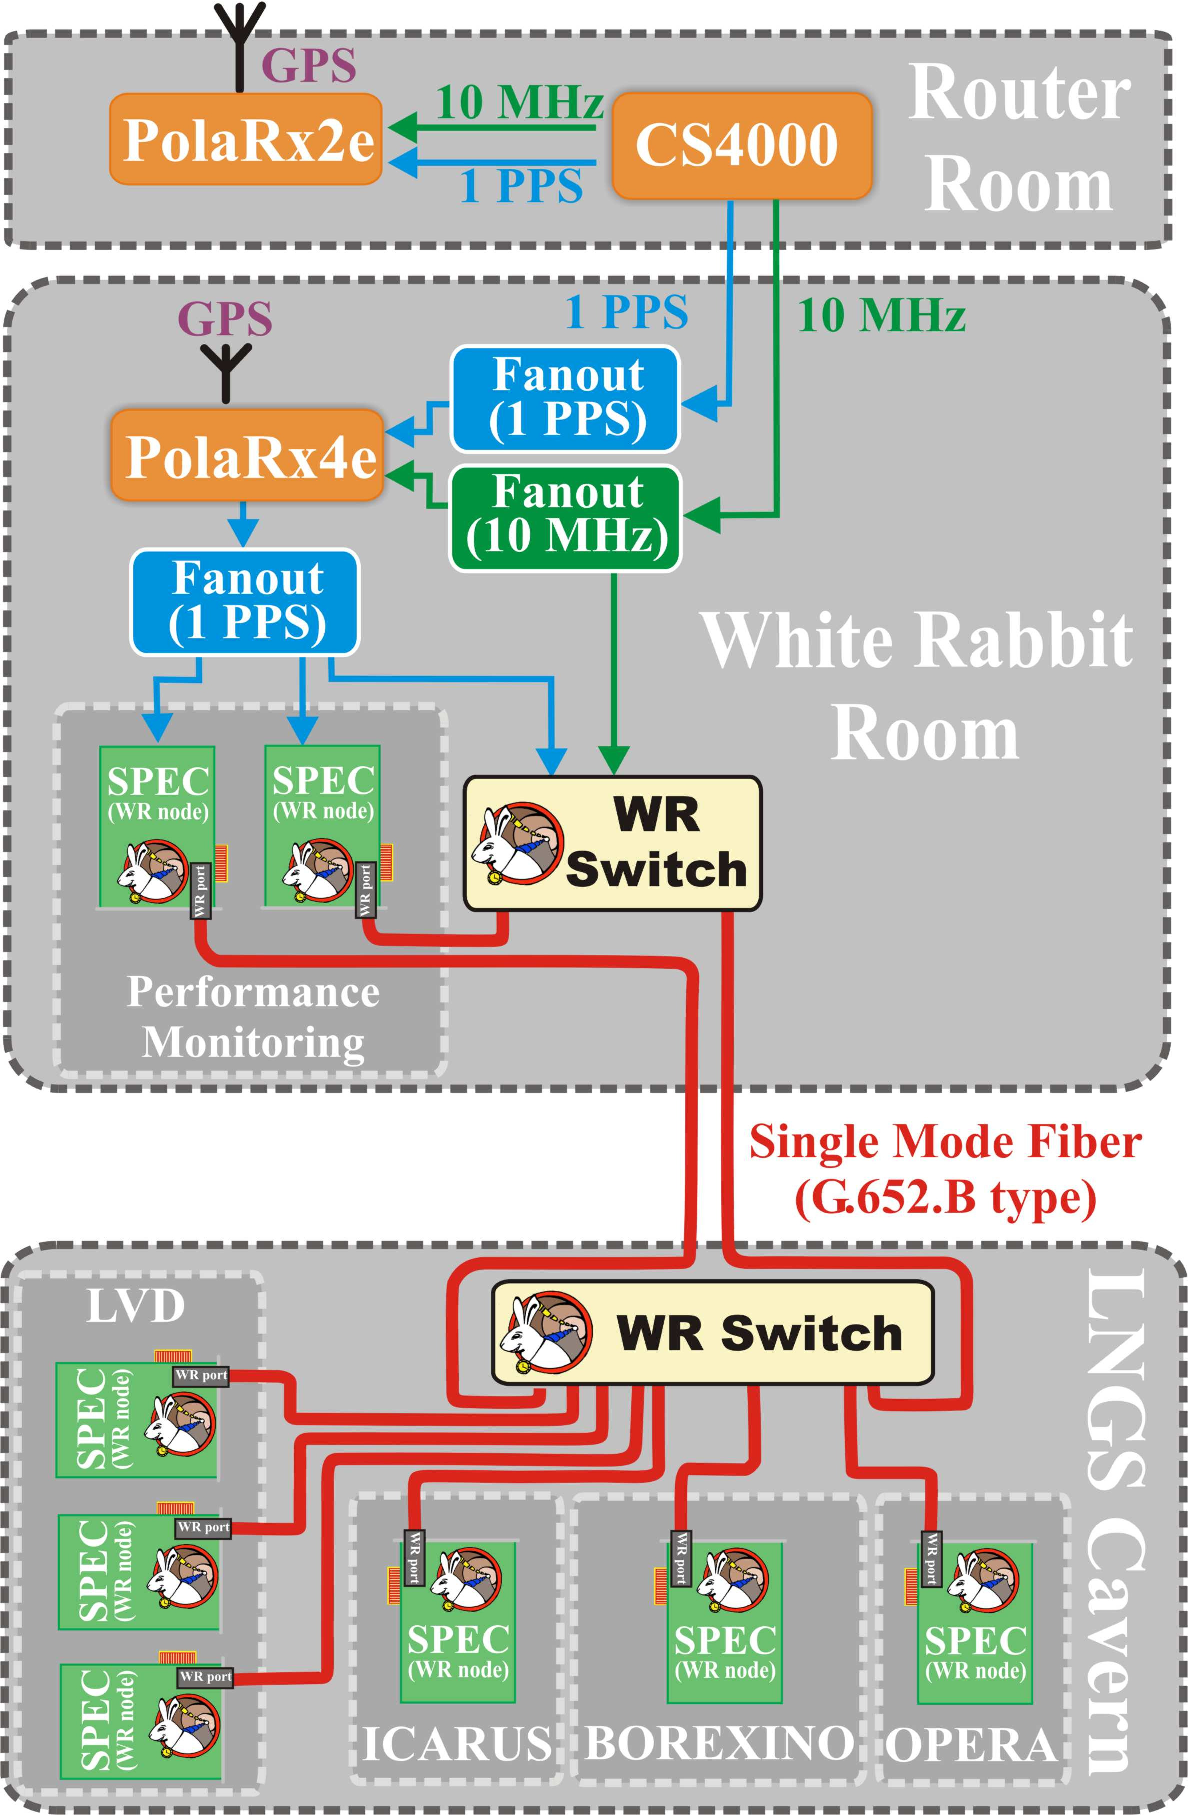
\includegraphics[height=4.0in]{applications/CNGS2.pdf}
\caption{White Rabbit based synchronization system in Gran Sasso National Laboratory (LNGS).}
\label{fig:wrLNGStiming}
\end{figure}

In the new WR installation (\figurename~\ref{fig:operaTiming} and \figurename~\ref{fig:wrLNGStiming}), 
a common UTC timebase for both remote sites is achieved using two 
identical systems, composed of a Septentrio PolaRx4TR \cite{biblio:PolaRx4e} GPS receiver 
operating in ``common-view" mode and a Symmetricom Cs4000 \cite{biblio:CS4000} Cs atomic clock, 
installed at CERN and LNGS. The Cs atomic clock is a common part of the new and the old 
time transfer systems. 

\figurename~\ref{fig:wrLNGStiming} details the WR setup in LNGS. The Septentrio PolaRx4TR 
accepts the GPS signal and the high stability CS4000 10~MHz signal to generate a timebase whose 
offset with respect to the GPS time can be \modified{derived} 
%known 
a posteriori with very good accuracy. 
The 10~MHz signal of the \modified{Cs atomic} clock (CS4000, installed in the {\it Router Room}) 
is connected (through a fanout) to the 
grandmaster switch. Thus, the timebase of the WR network is that of the  \modified{Cs atomic} clock, 
which in turn, 
can be directly translated to the GPS timebase. The grandmaster in the {\it White Rabbit Room} 
is connected through 8.3~km of fiber to the switch installed in the laboratory cavern. 
This switch serves as a \modified{fanout}
%hub 
for the nodes (SPECs) used in different LNGS experiments (i.e. LVD, 
OPERA, Borexino and ICARUS) as depicted in \figurename~\ref{fig:wrLNGStiming}. 
It is foreseen to extend this very simple network with more switches, possibly 
one for each experiment. 

%\figurename~\ref{fig:wrCERNtiming} presents a very similar WR setup for CERN installation. 

\subsection{Monitoring setup}

The timing performance of the WR installations is carefully monitored.
The PPS output 
of the grandmaster's time source is timestamped by two SPECs 
(\figurename~\ref{fig:wrLNGStiming}). One of the 
SPECs (called \textit{local SPEC}) is connected (through a short fiber) directly to the grandmaster switch (in WR Room), 
thus time-tagging the time source's PPS in 
the time referenced to the grandmaster. The second SPEC (called \textit{loopback SPEC}) 
is connected through 8.3~km of fiber to the 
second switch (located in the cavern), thus time-tagging the time source's PPS in the time 
referenced to the first-layer switch (boundary clock). This SPEC acts as a system loopback which 
provides an estimate of the quality of the time transfer to the SPECs used to time-tag
the input signals in each experiment. The total distance of the loopback is over 16~km 
(\modified{grandmaster $\rightarrow$ boundary clock $\rightarrow$ SPEC}). 


% Additionally, the 10MHz clock outputs of both 
% monitoring SPECs and the cesium clock are analyzed with Agilent E5052B signal source analyzer to
% measure the phase noise, L(f), and estimate the rms jitter.

% In order to compare and monitor differences between the new and the old systems, a PPS signal 
% generated by the old system is time-tagged (SPEC (2) in \figurename~\ref{fig:operaTiming}).

The temperature in the WR Room (in which the SPECs and the grandmaster switch are installed) as well
as the temperatures of the SPECs and Fine Delay modules are monitored. 

% The WR installation at CERN features additionally a roll of 
% fiber exposed to varying external condition (i.e. temperature)\footnote{Data from this setup not available at the time of writing.}. The variation of temperature 
% is logged. The SPEC node, connected to this fiber roll, time-stamps the PPS output of the 
% cesium clock while the 10MHz output of the SPEC is also analyzed with the Agilent device. 


\subsection{Temperature test setup}
\label{sec:tempTestSetup}

%Additionally to 
\modified{Aside from} monitoring the performance and parameters of the deployed system, 
a similar setup was tested in a CTS Climatic Chamber (Type T-40/500) to determine influence 
of the temperature variation on the %system's 
\modified{synchronization} performance. In this setup, a switch acting as a 
free running grandmaster was connected through 11~km of fiber to another switch acting as 
a boundary clock. One SPEC (called \textit{local}) was connected through 10~m of fiber to 
the grandmaster switch. Another SPEC (called \textit{loopback}) was connected to the boundary clock 
switch through 5~km of fiber. \modified{The boundary clock was connected to the grandmaster switch through 11~km 
of fiber.} The skews between the clock of the grandmaster switch and that of 
the boundary clock switch, the \textit{local} SPEC and the \textit{loopback} SPEC were measured using 
LeCroy WavePro 7300A oscilloscope. Monitoring the skew of the recovered clocks
(unlike \mbox{timestamping} the PPS reference) allows to evaluate the performance of the WR-timebase without
additional jitter or inaccuracy introduced by a system using the WR-timebase 
(i.e. TDC on the Fine Delay). 

Different elements of the described setup were placed in the climatic chamber while the rest 
of the setup was placed in a reasonably stable conditions of the laboratory (ambient temperature 
of 26$\pm$1.5 degrees Celsius). 

A temperature cycle consisted of ramping the temperature from 20 to 50 degrees, stabilizing 
at 50 degrees, ramping down to 0 degrees, stabilizing at 0 degrees and ramping up back to 20 degrees. 


% \begin{figure}[!t]
% \centering
% \includegraphics[height=2.0in]{fig/wrCERNtiming.ps}
% \caption{TODO}
% \label{fig:wrCERNtiming}
% \end{figure}






\section{Data Analysis}
\label{sec:dataAnalysis}


\subsection{Basic parameters of the deployed WR-based system}

\attention{The analyzed data consists of two sets of 2706160 \mbox{timestamps} collected over an undisturbed
system run of 31~days, 7~hours, 42~minutes and 40~seconds (Fri, 18 May 2012 22:38:53 GMT to 
Tue, 19 Jun 2012 06:21:33 GMT). The data was logged by the two SPECs (\textit{local} 
and \textit{loopback}) which used Fine Delay modules for timestamping the PPS reference signal 
(\figurename~\ref{fig:wrLNGStiming}).}
An extract from the timestamp logs is presented in Table~\ref{tab:rawData}. A visual inspection of the raw data 
shows a constant offset with respect to the reference PPS edge which occurs at \attention{0 nanoseconds}. 
This offset can be attributed to the different lengths of the cables connecting 
the reference PPS outputs to the inputs of the SPECs and that of the grandmaster switch as well as 
the internal delays of the switch locking to the reference PPS and the 10~MHz clock. 

% Importantly, the offset is the same for timestamps from both SPECs (\textit{local and loopack}) to within 
% instability which is the subject of further analysis.

The values of the Time Error (TE) were derived from the raw data by calculating the difference 
between a timestamp and an ideal PPS (occurring at \attention{0 nanoseconds}) and removing the average offset. 
The TEs for the \textit{local} and \textit{loopback} SPEC measurements are denoted $x_{lo}$ 
and $x_{lb}$ respectively (Table~\ref{tab:notRawData}). The performance of the system 
(two switches, two fiber links of 8.3~km each and two SPECs) can be characterized by calculating the 
difference (TE) between the corresponding timestamps from both SPECs, denoted $x_{diff}$ 
(Table~\ref{tab:notRawData}). The value of $x_{diff}$ with the average offset removed is \modified{denoted} 
$x_{diff-offset}$. 

% The TE values ($x_{lo}$, $x_{lb}$, $x_{diff}$ and $x_{diff-offset}$) 
% are used in this analysis to derived parameters of the deployed system. 

\begin{table}[!t]
\caption{Analyzed timestamps -- raw data}
\centering
\begin{tabular}{| l | c| c | c | c |}          \hline
& \multicolumn{2}{|c|}{\textbf{Local PPS }}  &  
\multicolumn{2}{|c|}{\textbf{Loopback PPS}}   \\   \hline
& \textbf{UTC} & \textbf{nanoseconds} & \textbf{UTC} & \textbf{nanoseconds} \\   \hline

1       & 1337380733 & 999999885.959 & 1337380733 & 999999885.500 \\   \hline
2       & 1337380734 & 999999886.014 & 1337380734 & 999999885.285 \\   \hline
3       & 1337380735 & 999999885.934 & 1337380735 & 999999885.338 \\   \hline
4       & 1337380736 & 999999885.906 & 1337380736 & 999999885.420 \\   \hline
...     &      ...   &  ..           &     ..     &      ..       \\   \hline
2706160 & 1340086893 & 999999885.879 & 1340086893 & 999999885.258 \\   \hline
         
\end{tabular}
\label{tab:rawData}
\end{table}

%\begin{table}[!t]
%\caption{Analyzed timestamps -- raw data}
%\centering
%\begin{tabular}{| l | c| c | c | c |}          \hline
%& \multicolumn{2}{|c|}{\textbf{Local PPS }}  &  
%\multicolumn{2}{|c|}{\textbf{Loopback PPS}}   \\   \hline
%& \textbf{UTC} & \textbf{nanoseconds} & \textbf{UTC} & \textbf{nanoseconds} \\   \hline
%
%1    & 1336823054 & 999999885.947266 &  1336823054 & 999999885.460938 \\   \hline
%2    & 1336823055 & 999999885.785156 &  1336823055 & 999999885.460938 \\   \hline
%3    & 1336823056 & 999999885.757812 &  1336823056 & 999999885.353516 \\   \hline
%4    & 1336823057 & 999999886.027344 &  1336823057 & 999999885.433594 \\   \hline
%...  &  ... & .. & .. & .. \\   \hline
%3719 & 1336826772 & 999999885.730469  & 1336826772 & 999999885.136719 \\   \hline
%\end{tabular}
%\label{tab:rawData}
%\end{table}


\begin{table}[!t]
\caption{Time Errors (TEs)}
\centering
\begin{tabular}{| l | c| c | c | c |}          \hline
& \textbf{$x_{lo}$} & \textbf{$x_{lb}$} & \textbf{$x_{diff}$} & \textbf{$x_{diff-offset}$}\\   \hline
       & [ns]  &  [ns]  & [ns]  &  [ns]  \\   \hline
1      & 0.043 & -0.015 & 0.459 & -0.058 \\   \hline
2      &-0.172 &  0.040 & 0.729 &  0.212 \\   \hline
3      &-0.119 & -0.040 & 0.596 &  0.079 \\   \hline
4      &-0.037 & -0.067 & 0.486 & -0.031 \\   \hline
...    &  ...  &  ...   &  ...  &  ...   \\   \hline
2706160&-0.037 & 0.0671 & 0.621 & 0.104 \\   \hline
\end{tabular}
\label{tab:notRawData}
\end{table}

\begin{figure}[!t]
\centering
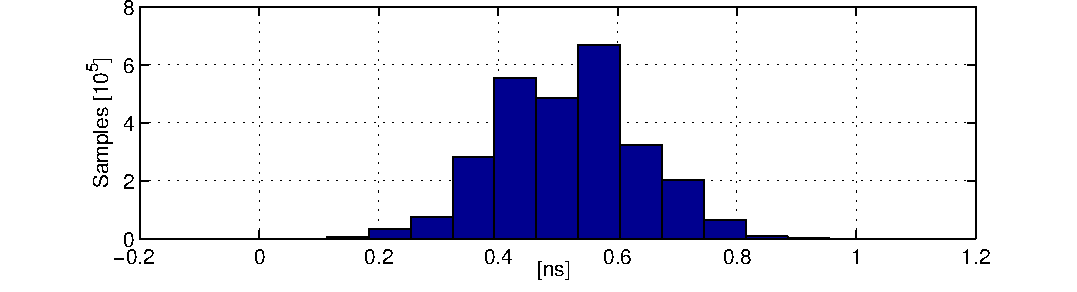
\includegraphics[width=0.5\textwidth]{../../figures/measurements/histogram-small.eps}
% \caption{A plot of the Time Error data with removed offset
% ($x_{lo}$, $x_{lb}$ and $x_{diff-offset}$) and a histogram of the difference between timestamps 
% acquired by the two SPECs ($x_{diff}$) which reflects system's performance.}
\caption{A histogram of the difference between timestamps 
acquired by the two SPECs ($x_{diff}$) which reflects system's performance.}
\label{fig:teAndHist}
\end{figure}


% \figurename~\ref{fig:teAndHist} presents a histogram of difference TE values ($x_{diff}$).
% Analysis of $x_{diff}$ are used to evaluate system accuracy and precision i.e. 

\figurename~\ref{fig:teAndHist} presents a histogram of $x_{diff}$ distribution. 
The average value of $x_{diff}$ marks the accuracy of the system and amounts to 0.517~ns
while the standard deviation of $x_{diff}$ reflects its precision which is 0.119~ns.
It is important to remember that these values include timestamping inaccuracy of the 
Fine Delay \cite{biblio:fineDelay} module (i.e. std. dev of 55~ps). 
% \attention{Therefore, 
% the numbers need to be understood as the characteristics of a complete system.}
The standard deviations calculated for $x_{lo}$ and $x_{lb}$ are 0.129~ns and 
0.125~ns respectively.

The Overlapping Allan Deviation calculated from the collected data is presented in 
\figurename~\ref{fig:oADEV}. The plot indicates White or Flicker PM Noise. 

\begin{figure}[!t]
\centering
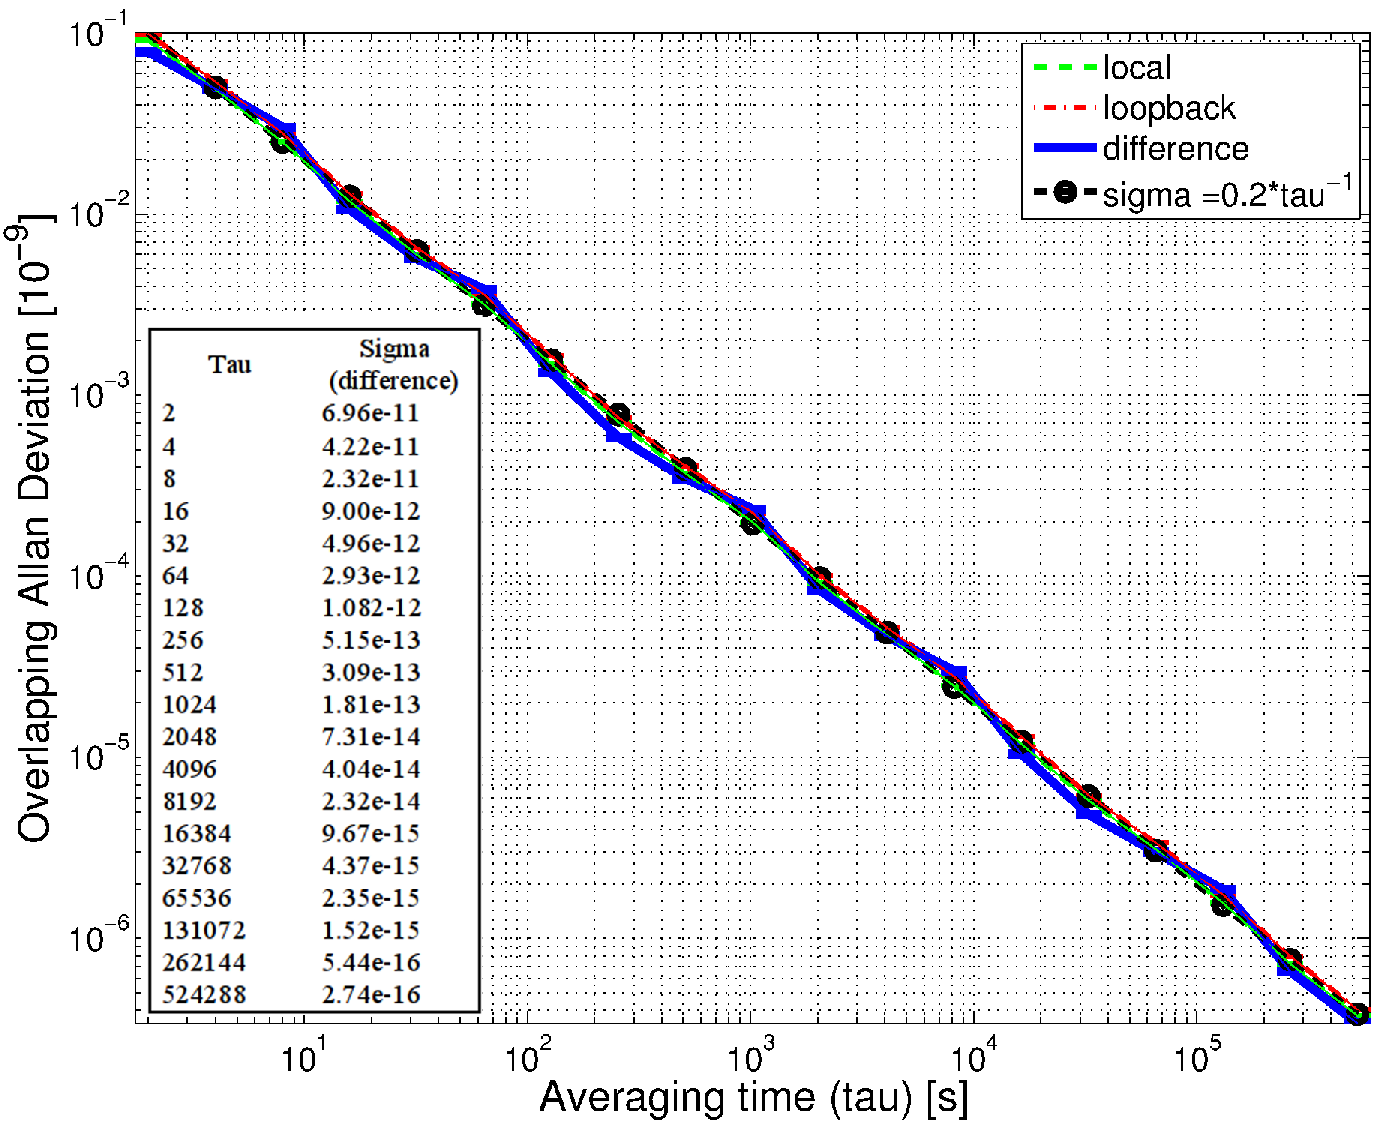
\includegraphics[width=0.4\textwidth]{../../figures/measurements/cngs_oADEV3.eps}
\caption{Overlapping Allan Deviation.}
\label{fig:oADEV}
\end{figure}

% The Maximum Time Interval Error (MTIE) presented in \figurename~\ref{fig:MTIE-no-cor} shows worse 
% performance of the \textit{local} SPEC compared to the \textit{loopback} SPEC. Removal of 9
% outliers from the \textit{local} SPEC data gives a more reasonable MTIE graph presented in
% \figurename~\ref{fig:MTIE-cor}. The cause of the outliers requires further investigation but it
% seems reasonable to suspect hardware or setup problem of the \textit{local} SPEC.  
% The Maximum Time Interval Error (MTIE) presented in \figurename~\ref{fig:MTIE-cor} proves the sub-nanosecond 
% performance of the system within the measurement period. The MTIE of $x_{diff}$ stabilizes at 
% around 0.95ns for the observation window values:
% \begin{equation}
%   \label{eq:mtie}
%   \approx 2048s (34min) < tau < 464074s (128.91h)
% \end{equation}
% 
% More data is highly desired to analyze a long term performance. 

The Maximum Time Interval Error (MTIE) of $x_{lo}$, $x_{lb}$ and $x_{diff-offset}$ 
was calculated for windows of $N_{tau}=2^k$ samples (k=1,2,3,...,21) and a window of the entire 
set of 2706160 samples. An optimized algorithm for MTIE
computation, called boundaries decision method \cite{biblio:MTIE}, was used to process 
\attention{the considerable number of samples in a reasonable time.}
The obtained MTIEs, depicted in \figurename~\ref{fig:MTIE},
indicate that the peak time deviations of the measured PPS signals (blue and green) are less than 1.15ns. 
However, the peak deviation between the two PPS measurements (blue) is smaller by 100ps 
(below 1.05~ns). It is important to mention that out of over 
2 millions measurements, only 9 values of $x_{diff-offset}$, 25 values of $x_{lo}$ and 146 values of 
$x_{lb}$ exceeded the $\pm$0.5~ns range. This constitutes 
0.0003$\%$, 0.0009$\%$ and 0.005$\%$ of the collected data respectively. The fact that the 
MTIE of $x_{diff-offset}$ is lower than the MTIEs of $x_{lo}$ and $x_{lb}$ might indicate 
external factor(s) affecting the entire system (thus removed with differential measurement) such
as temperature fluctuation.


\begin{figure}[!t]
\centering
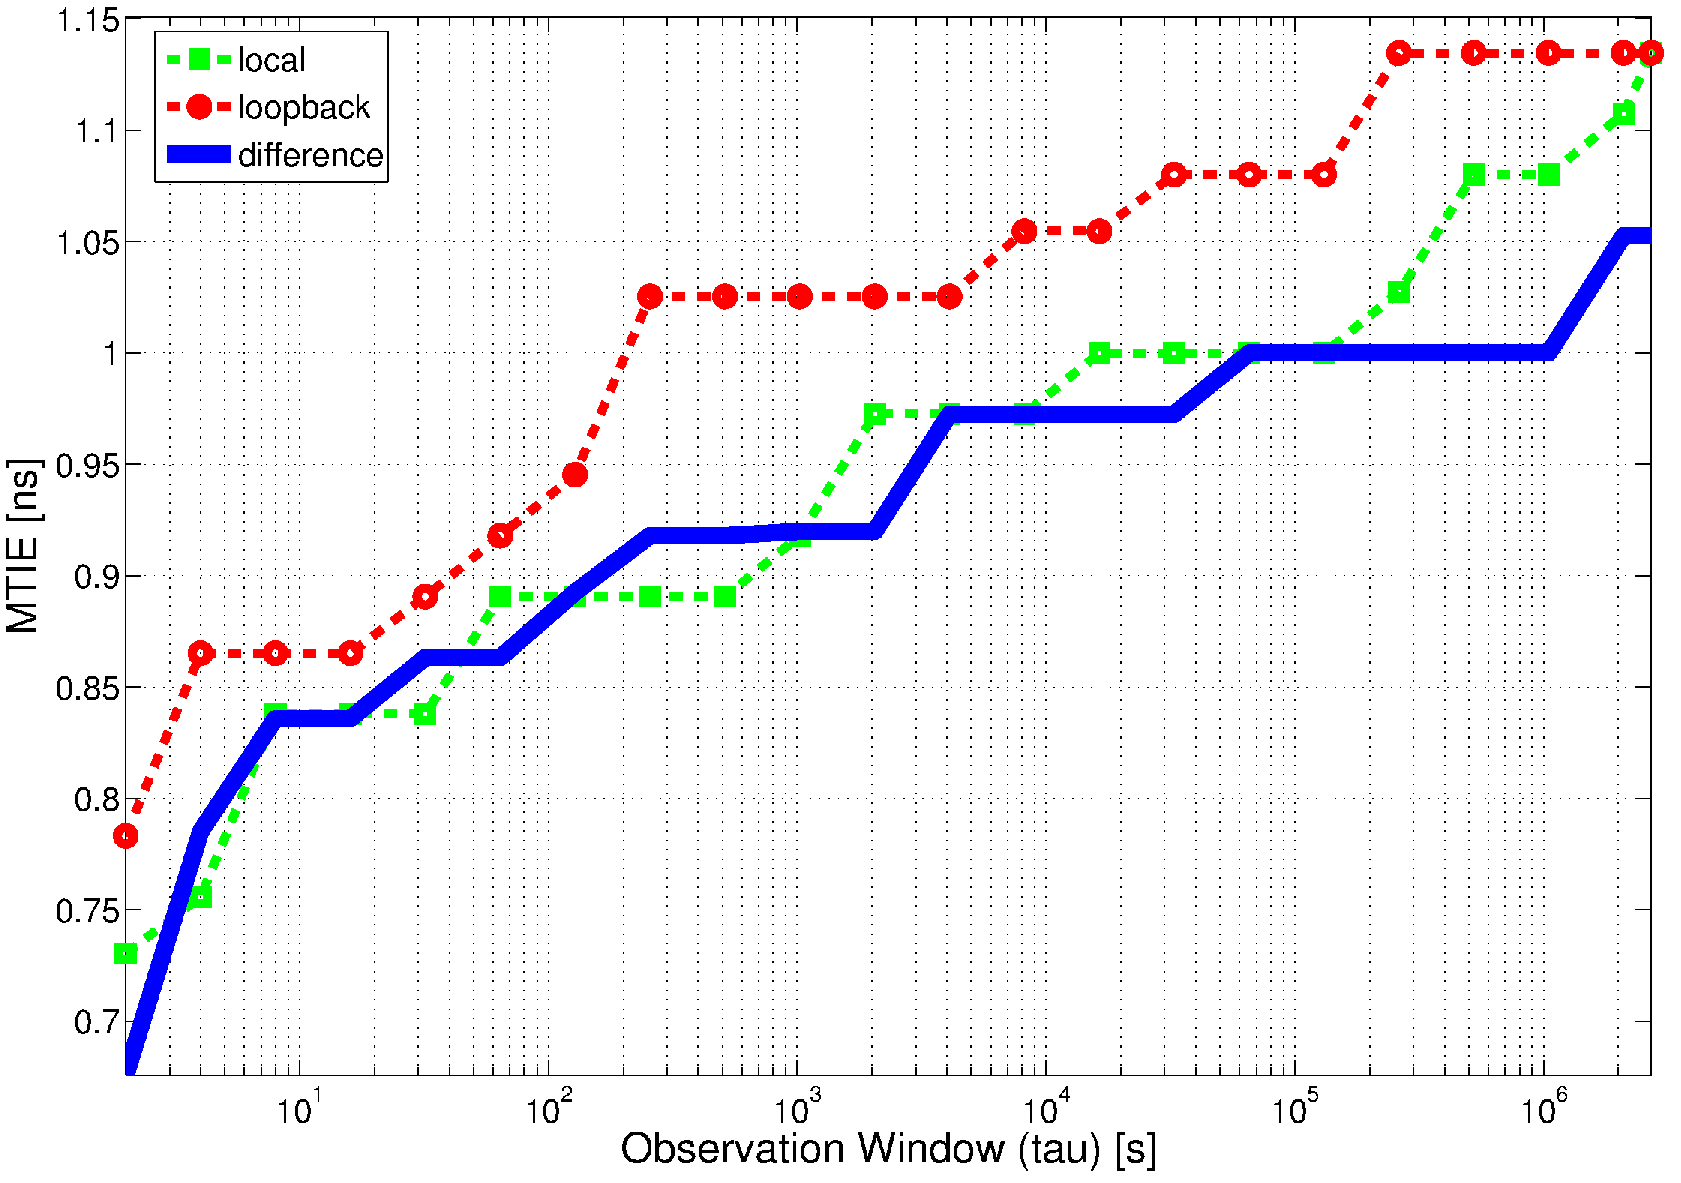
\includegraphics[width=0.4\textwidth]{../../figures/measurements/MTIE2.eps}
\caption{Maximum Time Interval Error (MTIE).}
\label{fig:MTIE}
\end{figure}

\subsection{Influence of temperature on the deployed WR-based system}

The temperature in the WR Room (\figurename~\ref{fig:wrLNGStiming}), where the grandmaster
switch and two monitoring SPECs are located, was logged over a substantial
part of the system run (Fri, 25 May 2012 14:00:00 GMT to Tue, 19 Jun 2012 06:00:00 GMT).
This temperature changed by 3.5 degrees Celsius over 25 days of observation time and 
a fraction of a degree on a daily basis, as depicted in \figurename~\ref{fig:temp.vs.TE} 
\modified{(upper plot)}. 
The blue sinusoid in the plots of \figurename~\ref{fig:temp.vs.TE} represents day-night cycles where the maximum indicates 
12:00 (local time) and minimum indicates 00:00 (local time). The lower plot of \figurename~\ref{fig:temp.vs.TE}
shows differential TE values ($x_{diff}$) which do not reveal noticeable changes with temperature. 

\begin{figure}[!t]
\centering
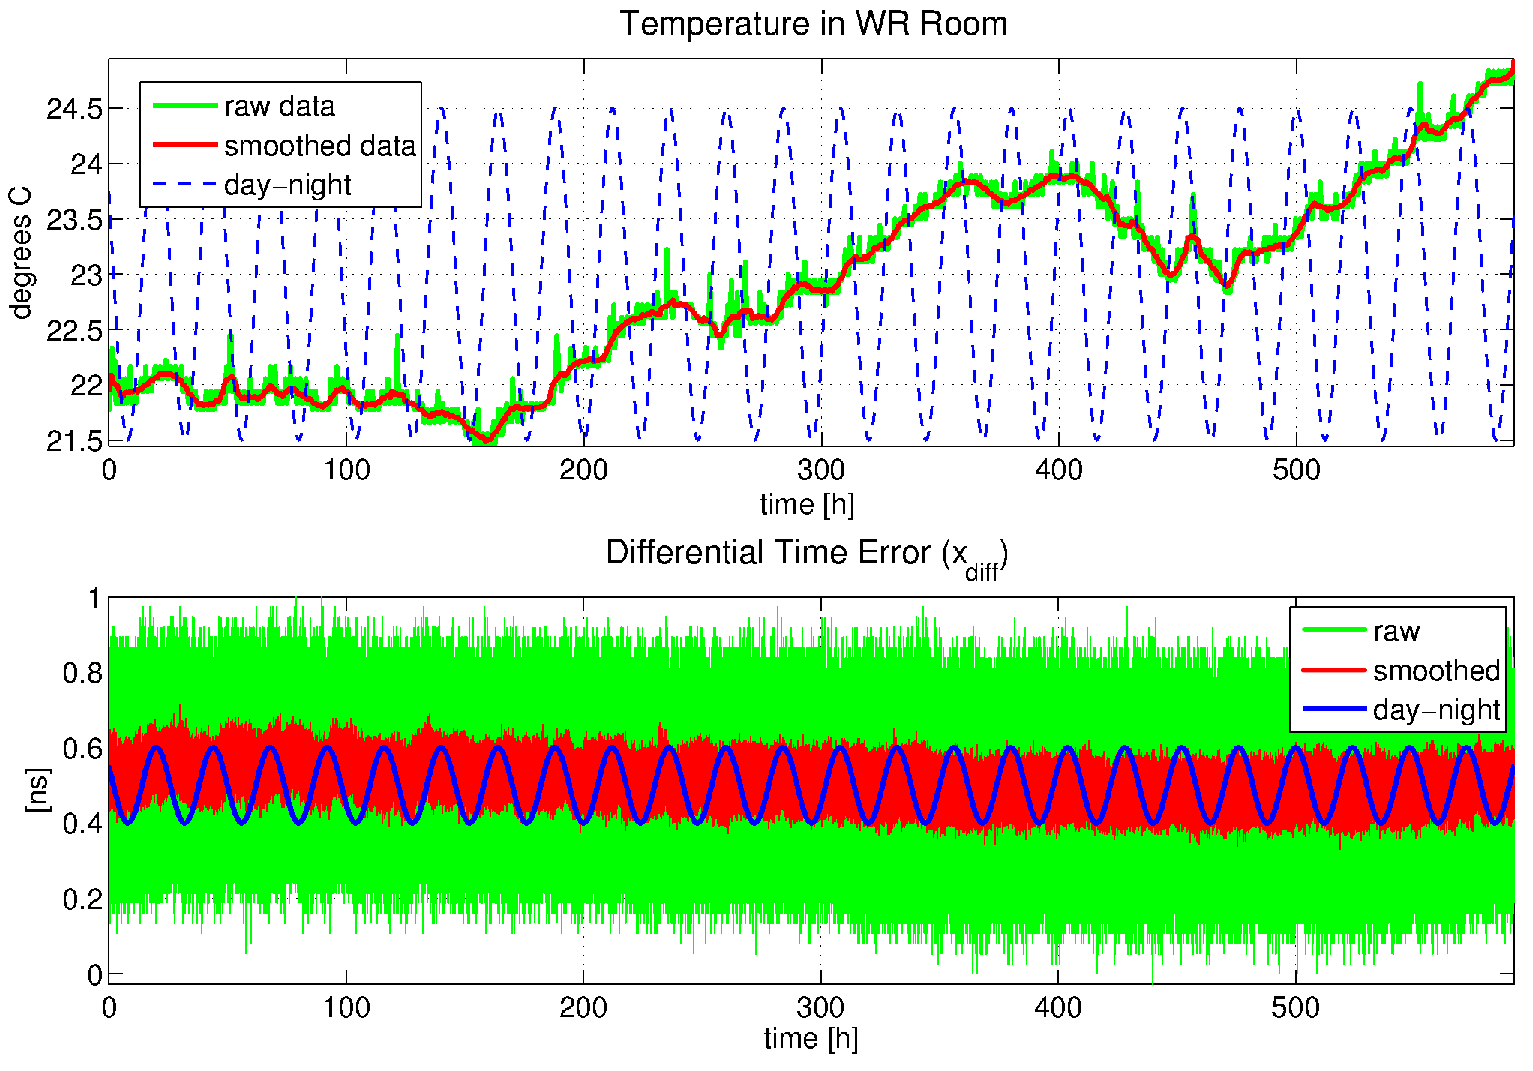
\includegraphics[width=0.4\textwidth]{../../figures/measurements/cngs_temp.vs.TE.eps}
\caption{Time Error versus temperature in WR Room.}
\label{fig:temp.vs.TE}
\end{figure}

Application of a 30 minutes-based averaging filter and smoothing of the raw data 
\modified{($x_{diff}$, $x_{lo}$ and $x_{lb}$)} enables to observe 
\modified{(\figurename~\ref{fig:temp.vs.filteredTE}, lower plot)}
a clear correlation between fluctuation of both SPECs' timestamps. The red line in 
\figurename~\ref{fig:temp.vs.filteredTE} (lower plot) shows fluctuation of timestamps measured by the 
\textit{local} SPEC \modified{($x_{lo}$)} while the blue line shows the fluctuation of the timestamps measured by the 
\textit{loopback} SPEC \modified{($x_{lb}$)}. Both lines
are correlated with a changing offset ($x_{diff}$) marked with the black line. For clarity,
WR Room temperature is depicted in the upper plot of the figure. The 
long-term oscillation of the differential TE ($x_{diff}$ in black) is not correlated 
with the temperature in the WR Room as the temperature keeps increasing while the 
$x_{diff}$ does not keep decreasing.
\figurename~\ref{fig:temp.vs.filteredTE} might indicate two sources of TE 
($x_{lo}$ and $x_{lb}$) fluctuation: (1) fluctuation of the entire WR-timebase with respect
to the reference PPS or (2) similar error introduced by the Fine Delay modules placed in the 
same location due to similar temperature variations.
The temperature monitored on the Fine Delay modules is stable to within 1 degree Celsius. Therefore,
\attention{the observed simultaneous fluctuation of both SPEC measurements} is most probably attributed to a factor not 
related with WR network (e.g. 10~MHz Fanout, \figurename~\ref{fig:wrLNGStiming}).

\begin{figure}[!t]
\centering
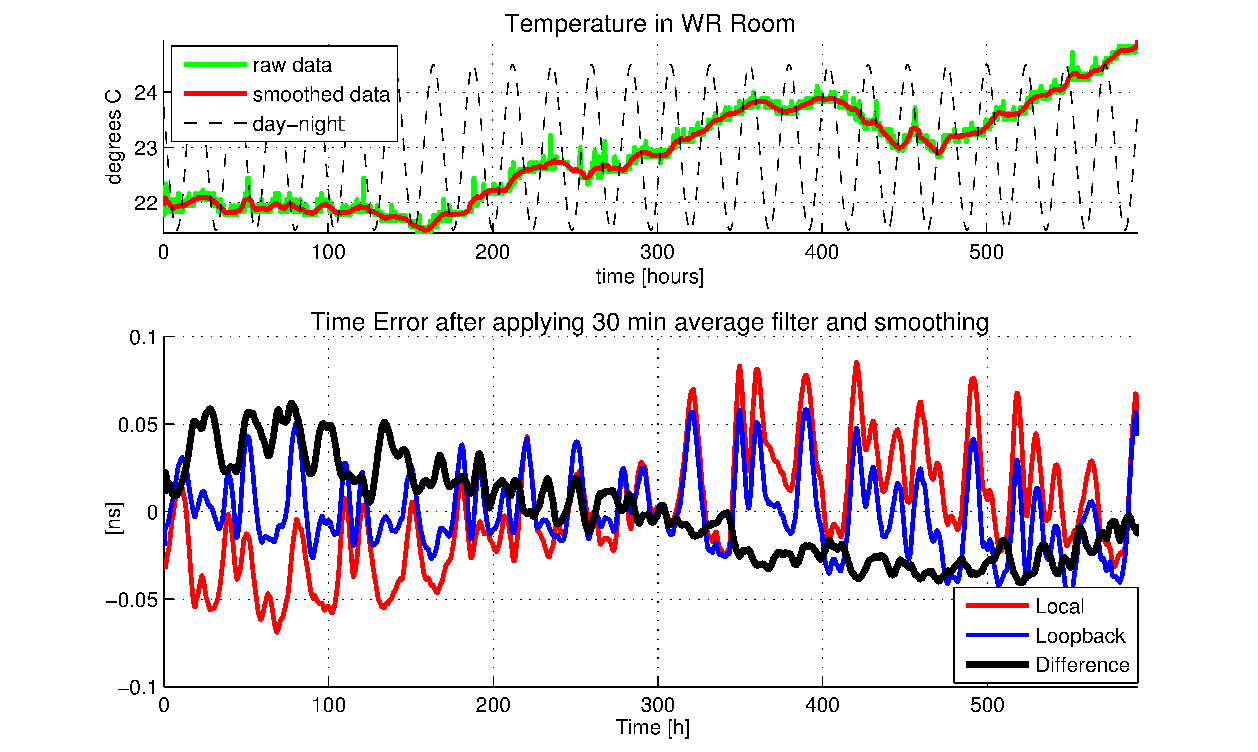
\includegraphics[width=0.5\textwidth]{../../figures/measurements/cngs_temp.vs.filteredTE3.eps}
\caption{Time Error (after applying 30 min average filter and smoothing) versus temperature in WR Room.}
\label{fig:temp.vs.filteredTE}
\end{figure}

% \begin{figure}[!t]
% \centering
% \includegraphics[width=0.5\textwidth]{newFig/temp.vs.FD.eps}
% \caption{Time Error versus temperature in WR Room and on the Fine Delay (~23 July 20 to ~11:30 July 22).}
% \label{fig:temp.vs.FD}
% \end{figure}


\subsection{Influence of temperature on the WR-timebase}

The temperature of the described and monitored WR-based system in LNGS is very stable. 
The temperature of the WR Room
shows small long-term drift of 3.5 degree Celsius. The boundary clock switch 
is installed in a cavern in the heart of a mountain and its temperature is supposedly considerably 
stable, though no temperature measurement is available. The fluctuation of the fiber's temperature 
is estimated at around 0.4 degrees Celsius. 

However, the SPEC cards used by the different LNGS experiments 
(\figurename~\ref{fig:wrLNGStiming}) might be subject to varying temperature. 
Furthermore, \attention{in many of the future applications} of WR-based systems (e.g. HiSCORE-EA at the Tunka 
in Siberia \cite{biblio:tunka} or LHAASO in Tibet \cite{biblio:LHAASO}) the nodes will be subject 
to a wide range of temperatures while the switches will be in reasonably stable
temperature conditions.

Therefore, in order to discriminate the influence of varying temperature conditions of a 
WR Node (i.e. SPEC) on the WR-timebase quality, a similar setup to the one 
deployed in LNGS was tested in a climatic chamber (described in Section \ref{sec:tempTestSetup}). 
The following parameters were monitored:
\begin{itemize}
  \item Temperature in the climatic chamber
  \item Temperature on each SPEC
  \item Skew between the clock of the grandmaster switch (time reference) and the clocks recovered 
        on each SPEC
\end{itemize}
% The cable round trip is obtained using values of the four timestamps:
% \begin{equation}
%   \label{eq:delaymm}
%   delay_{MM} = (t_{4p}-t_{1}) - (t_{3}-t_{2p})
% \end{equation}
% and subtracting the values (measured by WRPTP) of hardware delays between the timestamping point in 
% FPGA and the SFP optical in/out. This value represents the best estimate of the delay introduced
% by the physical link (i.e. fiber) and is used to calculate one-way master-slave delay by applying
% relative delay coefficient (know for a given medium) to compensate for the medium's asymmetry.

\begin{figure}[!t]
\centering
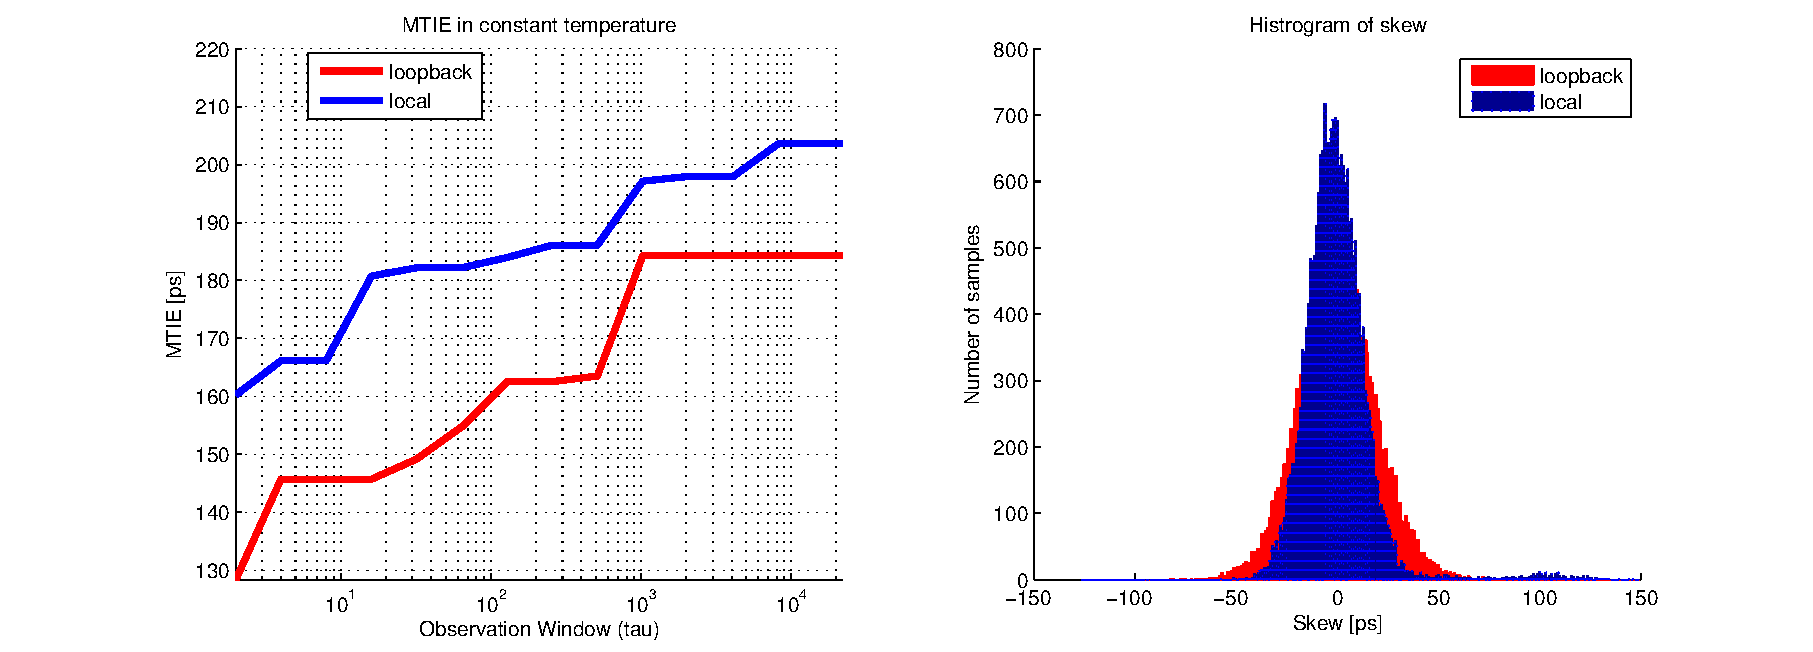
\includegraphics[width=0.5\textwidth]{../../figures/measurements/cngs_reference.eps}
\caption{\textbf{TEST 1}: parameters of the system in constant temperature (20 degrees Celsius).}
\label{fig:chamber-ref}
\end{figure}
% 

Firstly, the performance of the system was evaluated in a temperature-stabilized conditions of 
20 degrees Celsius. The measured 
system parameters are depicted in the column \textbf{TEST~1} of Table~\ref{tab:dataCompare} and in 
\figurename~\ref{fig:chamber-ref}.


\begin{figure}[!t]
\centering
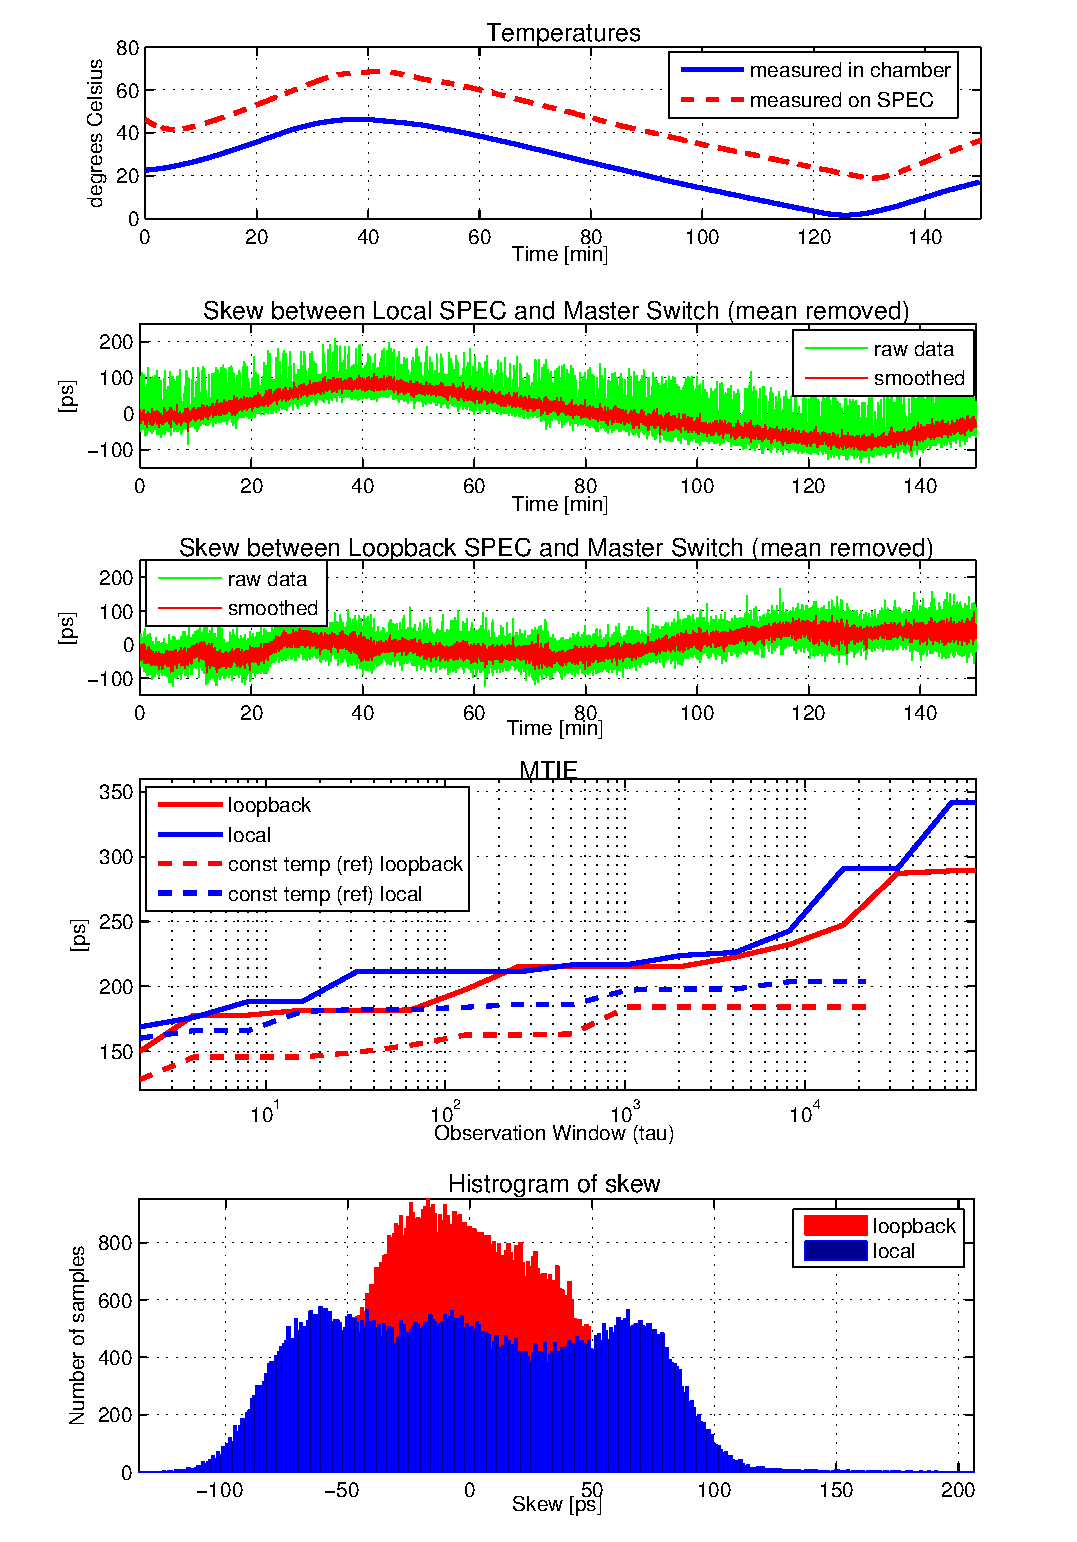
\includegraphics[width=0.5\textwidth]{../../figures/measurements/chamber-test.eps}
\caption{\textbf{TEST 2:} system performance when changing temperature of both SPECs.}
\label{fig:chamber-test}
\end{figure}


Secondly, both SPECs were placed in the climatic chamber while the rest of the setup
(i.e. two switches and fibers) were kept in the ambient temperature of the laboratory
(26$\pm$1.5~degrees Celsius). The test consisted of a single temperature cycle (described in
Section \ref{sec:tempTestSetup}) of 145 minutes. The measured system parameters are depicted in the 
column \textbf{TEST 2} of Table~\ref{tab:dataCompare} and in \figurename~\ref{fig:chamber-test}. 
The chamber's temperature (blue in the upper plot of
\figurename~\ref{fig:chamber-test}) as well as the SPEC's temperature (red) changed peak-to-peak
45 degrees Celsius. A fluctuation of the skew measured on the \textit{local} SPEC, depicted in the 
second plot in \figurename~\ref{fig:chamber-test},
is directly correlated with the temperature variation. This is due to the fact that the values of 
fixed delays (introduced by tx/rx hardware) compensated by the WRPTP protocol are assumed 
to be constant. This assumption holds for small temperature variation but introduces additional 
inaccuracy of synchronization over large temperature changes.
%, especially for short fibers. 
The skew of the \textit{loopback} SPEC (\figurename~\ref{fig:chamber-test}) is not directly 
correlated with the temperature.
However, it should be pointed out that the skew is measured between the \textit{loopback} SPEC and the 
grandmaster switch connected through another switch and a total of over 16~km of fiber. Therefore, what is 
observed in the plot is an addition of 
the temperature-induced fluctuation and a jitter introduced by the system (not related with 
temperature). \attention{Importantly}, the degradation
of the synchronization performance (depicted in MTIE plot in \figurename~\ref{fig:chamber-test}) 
over a considerable range of temperatures is reasonably small and does not prevent
the system from providing a sub-nanosecond synchronization accuracy and precision in the order of tens 
of picoseconds. 

Moreover, the clearly linear dependency between the variation of the temperature and that of the 
hardware delays can be easily compensated e.g. by providing a model of delays changes 
and applying their different values based on the temperature measurement from the SPEC's (or switch's) 
thermometer.


\begin{table}[!t]
\caption{Measured parameters of WR system during temperature tests}
\centering
\begin{tabular}{| l | c| c | c | c |c|}          \hline
                        &\textbf{TEST 1} & \textbf{TEST 2} \\   \hline
\textit{local} SPEC skew sdev [ps]    & 17             & 55              \\   \hline
\textit{loopback} SPEC skew sdev [ps] & 19             & 36              \\   \hline
\textit{local} SPEC MTIE         [ps] & $\leq$203            & $\leq$342             \\   \hline
\textit{looback} SPEC MTIE       [ps] & $\leq$184            & $\leq$289             \\   \hline
\end{tabular}
\label{tab:dataCompare}
\end{table} 

% 
% In the first test (TEST1) the performance of WR-timebase is evaluated in temperature-stabilized
% conditions with constant temperature of 20 degrees Celsius. The results are depicted in 
% \figurename~\ref{fig:chamber-ref} and included in Table~\ref{tab:dataCompare}.
% The performance of the WR-timebase in varying conditions is compared to the results in TEST 1. 
% 
% 

% \figurename~\ref{fig:chamber-test7} depicts results of the TEST 2 where the temperature of 
% the three fibers (10km, 5km and 10m) was changed over the time of 120 minutes. 
% It can be seen that the changes of the delay introduced by varying temperature are greatly 
% compensated. The skew of the local SPEC 
% is comparable with the one in the constant temperature (TEST 1). The skew of the loopback SPEC 
% increases in the order of 90ps (Table~\ref{tab:dataCompare}). The distribution of the loopback 
% skew is spread because of the addition of jitter introduced by both fibers (10km and 5km) 
% between the loopback SPEC and the grandmaster switch.
% 
% % \begin{figure}[!t]
% % \centering
% % \includegraphics[width=0.5\textwidth]{newFig/chamber-test7}
% % \caption{Climatic chamber test: changing temperature of fibers}
% % \label{fig:chamber-test7}
% % \end{figure}
% 
% 
% Variation of the temperature of the both SPECs in TEST 3 (\figurename~\ref{fig:chamber-test8}) 
% causes greater influence of the WR-timebase performance. The plot depicting the skew of 
% the local SPEC (\figurename~\ref{fig:chamber-test8}) clearly shows that the change of the
% hardware tx/rx elements of the SPEC causes skew fluctuation. The plot showing cable round trip 
% measurement explains what happens: the changes of the hardware delays (not compensated for) 
% causes virtual changes of the delay introduced by fiber, thus the non-existant change of 
% fiber temperature is compensated introducing decrease of synchronization precision. It is 
% worth noting that this effect is reasonably small for the tested range of temperatures (0-50
% degrees Celsius) and the MTIE is increased by less then 150 ps (Table~\ref{tab:dataCompare}).
% 
% Similarly, in TEST 4 the two switches were put into varying temperature conditions. The temperature
% variation of switches has substantially smaller effect on the performance of the local SPEC while
% substantially affects performance of the loopback SPEC. Still, the synchronization accuracy is 
% well within 1 ns. 
% 
% The last test, TEST 5, in which all the components of the system were put into varying conditions
% causes the comparable deterioration of the synchronization performance of the 
% WR-timebase. 



% \begin{table}[!t]
% \caption{Parameters comparison for different chamber test}
% \centering
% \begin{tabular}{| l | c| c | c | c |c|}          \hline
% TEST                    & \textbf{1} & \textbf{2} & \textbf{3} & \textbf{4}   & \textbf{5}\\   \hline
% local    skew sdev [ps] & 18         & 16         & 55         & 27           & 66 \\   \hline
% loopback skew sdev [ps] & 19         & 35         & 36         & 70           & 32 \\   \hline
% local MTIE         [ps] & 203        & 216        & 342        & 248          & 402 \\   \hline
% looback MTIE       [ps] & 184        & 275        & 289        & 442          & 322 \\   \hline
% \end{tabular}
% \label{tab:dataCompare}
% \end{table}

% All of the above tests show that the temperature variation of the WR system components has 
% direct effect on the synchronization performance of the system. However, the tests prove that
% the sub-nanosecond synchronization accuracy of the WR-provided timebase is guaranteed regardless
% of the temperature changes. 



\section{Conclusions}
\label{sec:conclusions}

In this paper the first deployment of a ``beta version" of a White Rabbit
system is described. The deployed system includes a WR Network (consisting of switches) 
interconnecting WR Nodes. 

The results indicate that a system based on the 
White Rabbit technology is capable of providing nanosecond accuracy of synchronization 
over large distances (i.e. over 16 km). The measured accuracy of the deployed system  
is 0.517~ns and the precision is 0.119~ns. The calculated MTIE is below 1.05~ns
with only 0.0003$\%$ of values exceeding the $\pm$0.5~ns range.
The WR-timebase 
guarantees sub-nanosecond accuracy and tens of picoseconds precision of the distributed time 
and frequency reference regardless of the changing temperature conditions. 
The standard deviation of the skew measured between the time reference (grandmaster) and 
the nodes (over a peak-to-peak 45 
degrees Celsius temperature range) is 55~ps while the MTIE is below 342~ps. 
The temperature tests indicate that the acceptable influence   
of the temperature variation of WR devices on the quality of synchronization can be easily
reduced by compensating temperature-induced changes of the hardware delays. 
Such a compensation should be considered in future developments of the WR technology.

The high accuracy and precision time transfer over an Ethernet-based WR Network has many potential
applications. Precise time-tagging of the input events using WR-provided timebase is the first to
be realized. Therefore, the described deployment marks an important milestone in the White Rabbit Project -- 
proof-of-concept technology becomes a working solution. This solution is about to be 
commercially available while sustaining its openness (open hardware and open software). 


\newpage

\bibliographystyle{IEEEtran}
\bibliography{IEEEabrv,./biblio}

\end{document}


